%\documentclass[11pt, oneside]{article}   	
%\usepackage{geometry}    
%\geometry{letterpaper}                 		
\input preamble.tex
\newcommand{\ig}[2][width=4in]{\includegraphics[#1]{#2}}    		
\usepackage{graphicx}					
\usepackage{amssymb}
\usepackage{pgfplotstable}
\usepackage{float}
\usepackage{caption}
\captionsetup[table]{justification=justified,singlelinecheck=false, position=bottom}
\begin{document}

\header {\today}							
\title{Muon Lifetime}
\author{Ekta Patel \& Brandon Booth-Dunbar}

\section{Abstract}
%Ekta
\begin{em} Positively charged muons reach the Earth via cosmic ray showers.When they decay, the muons break down into a positron, an electron neutrino and a muon neutrino.The goal of the experiment is to measure the lifetime of the muon by detecting and stopping a positive muon in an aluminium slab and then consequently detected the positron that it leaves behind when it decays.The distribution of the difference in detection times can be used to determine the muon lifetime.
\end{em}

\section{Theory}
%Brandon
\indent \indent Cosmic ray showers produce positively charged muons from $\pi$ meson decay high up in the atmosphere. While the half life of the $\mu^+$ is only around 2$\mu s$ relativistic time dilation results in a flux at sea level of around $1/cm^2/min$.  In this experiment we are interested primarily in the decay process of $\mu^+$ which is governed by the following equation:
\begin{equation}
	\mu^+ \rightarrow e^+ + \nu_e + \bar{\nu_e}
\end{equation}
\indent \indent As with most decays we can describe the decay probability as a function of time using a negative exponential of the form:
\begin{equation}
P_{decay}(t) = A e^{-\alpha t} + C
\end{equation}
\indent \indent \indent \indent where 
\begin{equation}
\alpha = \frac{1}{\tau}
\end{equation}
$\tau$ will be the mean lifetime of the decay particle. $A$ adjusts for the initial amplitude of the function depending on the data collected. $C$ will adjust for experimental background. 

\indent \indent The flux per a unit area can also be calculated in this experiment and is found by a relation between the number of events detected and the total time detectors were running. Then adjust for the area of the detectors to obtain a base unit value. 
\begin{equation}
\frac{Total\;Events}{Total\;Time}\; X\; \frac{1}{Detector\;Area} = \frac{Events}{Time\;Area}
\end{equation}



\section{Experimental Methods}
%Ekta, but I (Brandon)  will make the figures
\subsection{Apparatus}
\indent  \indent As a positively charged muon reaches the Earth and hits the scintillation detector, a small flash of light is observed due to the plastic sheet of the scintillator. The photomultiplier then changes the flash of light into a pulse of electrons which then travels to an amplifier/discriminator that filters away the noise from the detector in addition to strengthening the incoming pulse of electrons. The amplifier/discriminator then feeds the output pulse into the coincidence circuit to ensure that only the positrons and muon electrons are detected. 
\newline \indent We want to start a clock when a positive muon is detected in the aluminium slab and stop the clock when the positron is detected from the muon decay. The distribution of a very large number of delay times, created by the `start' and `stop' of the detections, will be used to determine the lifetime of the muon. 
\newline \indent In our setup, we have three photomultipliers($A, B, C$), two of which will trap the muon long enough for it to decay and a third that will help in the detection of the positron. We use the $A$ and $B$ photomultipliers to detect and trap the muon. When $A$ and $B$ are triggered, but not C, the clock will start to count until either $B$ or $C$ is triggered again by the positron and stops the clock. We do not want all three photomultipliers to be triggered when the muon is detected because the time delay will be irrelevant since the clock will start and stop almost instantaneously. We need the muon to be trapped by two photomultipliers and the resulting positron to be detected by one of the photomultipliers. Therefore, the start and stops of the clock correspond to:
\begin{equation} start: \textbf A\;and\; \textbf B \;sin\; \textbf C \end{equation}
\begin{equation} stop: \textbf B\; or\; \textbf C \end{equation}
Though we choose to setup our apparatus in this way, there is also another possibility in which the $A$ and $B$ photomultipliers are used to detect the muon but then only $B$ exclusively or C detect the positron ($B$ XOR $C$). This setup guarantees that the clock would only be stopped if either $B$ or $C$ were activated, but not both since the positron only travels either up or down through the apparatus as the muon decays. However, we do not choose to set up our experiment that way because it is not likely that another muon will be detected faster than in the time scales that we are observing. Since the muon realistically only takes about 2 $\mu$s to decay, a false trigger of photomultiplier $B$ would have to take place in that much time or less. During calibration, we find that $B$ receives about 50 counts per second. Therefore, it is triggered about 10$^{-4}$ times within the muon lifetime of approximately 2$\mu$s, making it nearly impossible to detect a muon in the same time span that one is already decaying. It is also important to remember that muons are only reaching the Earth's surface at a  muon sea level flux of only 1 /cm$^2$/minute or about one muon every 6x10$^7\mu$s.
\newline \indent As the photomultipliers are triggered, Time-to-Amplitude Converter converts the times between each `start' and `stop'  to voltages. These voltages are then recorded by the Multi-Channel Analyzer which uses the computer to bin the data into a histogram based on the strengths of voltages which correspond to the lengths of times taken for each detected muon to decay. It is important to remember that the muon flux at sea level is only 1 /cm$^2$/minute, so we will need to take data sets that stretch over several days to a few weeks to get a good distribution of delay times. A good representation of the apparatus from the photomultiplier tubes to the logic setup and ending with the final output of time delays is shown in the figure below: 


\begin{figure}[H]
\begin{center}
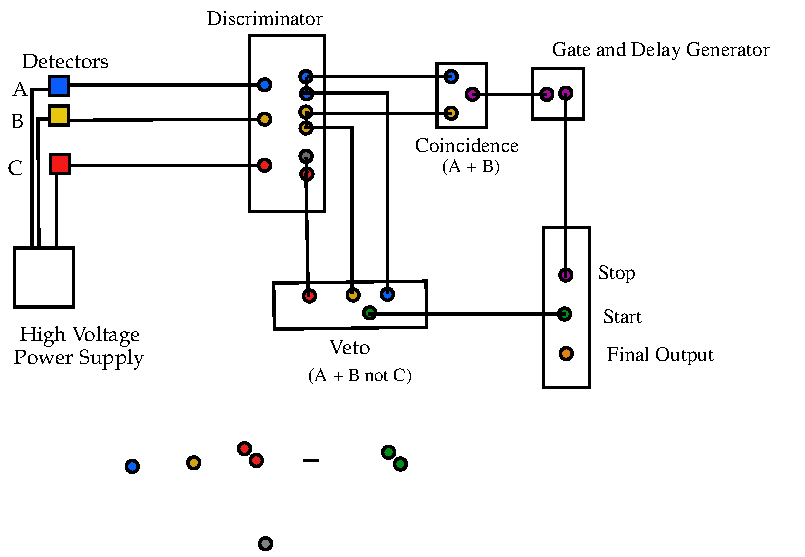
\includegraphics[width=6 in]{ML-figure1.pdf}
\caption{The apparatus}
\end{center}
\end{figure}

\subsection{Procedure}
\indent \indent To obtain the clearest and best signals possible for muon detection, we must first plateau each photomultiplier so that the signal to noise ratio of each one is as ideal as possible. The noise level will increase exponentially with time, whereas the signal will reach a maximum value and then plateau. This plateau region is the voltage that we want to achieve for photomultipliers A, B and C. We use an electron source of Bismuth to plateau the detectors by placing the source in approximately the same place on the aluminum slab leading to the photomultipliers while plugging in each one individually to the counter to see the counts detected just from the source's presence over one second time intervals. We started at a voltage of about 1000V for each of the photomultipliers and increased by 100V until we reached 1400V. At that point, we increased in increments of 10V as to not exceed the maximum voltage of 1500V. The table below gives the results of the voltages at which we found the plateaus in counts and the corresponding counts both with and without a source present. 
\begin{table}[h]
\begin{center}
\begin{tabular}{|c|c|c|c|} \hline
Photomultiplier & Voltage & Counts w/ Source & Counts w/o Source \\ \hline
A & 1450 V & 295 & 50 \\ \hline
B & 1450 V & 440 & 140 \\ \hline
C & 1470 V & 420 & 80\\ \hline

\end{tabular}
\caption{Values chosen for power supplied in voltage to each photomultiplier, including the number of counts with a Bismuth source on the apparatus to no source on the apparatus. The time interval for the number of counts for all three photomultipliers is 1 second.}
\end{center}
\end{table}

Data sets are taken on time scales of several days to a few weeks to obtain a result with reasonable precision. As discussed earlier, muons are not reaching the Earth at a very high rate, but furthermore, they are not being stopped in our apparatus 100\% of the time that they reach the ground. Therefore, longer time scales are more suitable to analyse the range of time delays that are used to determine the muon lifetime. After data has been obtained, it is important to calibrate the Time-Amplitude Converter to remove extraneous results that may be time delays that are too large to be feasible with the rest of the data set or even too small. The following table shows corresponding values for the amount of time lapsed in comparison to the matching bin number. The total number of bins observed with both the one week long and two week long data set is set to be 2048. Therefore, about 10\% of the total number of bins represent time delays of 1$\mu$s or less, whereas about 60\% of the bins correspond to time delays of 4$\mu$s or greater. 
\begin{table}[h]
\begin{center}
\begin{tabular}{|c|c|}\hline
Time & Bins\\ \hline
1 $\mu$s & 204.85\\ \hline
2 $\mu$s & 402 \\ \hline
3 $\mu$s & 608 \\ \hline
4 $\mu$s & 809 \\ \hline
\end{tabular}
\caption{Number of microseconds for which the calibration of the data has been determined to be binned. The number of bins given represents the number of bins from the zeroeth bin in our data run. The total number of bins  is 2048.}
\end{center}
\end{table}

% 2- 402 bins
% 3 -- 608
%4-- 809 bins over


\section{Results \& Discussion}
%Brandon
\indent \indent For this experiment we took two runs of data; the first for a 7 day interval and the second for 14 days.  The second run of data reached the maximum number of recorded events for the data collection program some time during the second week. In order to make it so that we can compare the two sets of data without knowing the relative total collection time we will divide by the total number of events in each data set and express the fit as a probability density function which gives us the percent chance of detecting an event with a certain decay time. It is usually best to express your results as intensive properties such as probability density functions because it allows for easy comparison to other data sources.\\
\indent \indent The output from the computer software used to gather data is given in the form of bins and counts.  The bin data set is a discrete integer ranging from 1 to 2048 and acts as a measure of the time-scale which we calibrated in the previous section.  The counts data set is the number of events that were recorded with a certain decay rate as indicated by the bin number.\\
\indent \indent In order to get the data ready for fitting we altered it in two ways:
\begin{enumerate}
\item There were a number of `dead' bins at the front of the data set which if left unaltered would skew the fit with outlier values.  In order to eliminate these bins we filtered our data for any bins in the first 200 that had corresponding count values of less than 10.  
\item We then further eliminated outliers in the data by establishing a variability threshold of $\pm \frac{moving-average}{2}$.  The moving average was computed over the 10 surrounding values.  Both increasing  the number of values used to compute the moving average as well as increasing the factor on the bottom will make this a more stringent criteria.
\end{enumerate}
\indent \indent After filtering the values in this manner we then converted our bins to the correct time scale using our calibration data given in Table 2 and normalized the counts portion by dividing by the total number of counts in the data set for the reasons outlined at the beginning of this section. Using this data we performed our exponential fit using Eq. 2. Our fit parameters were the inverse of the mean lifetime of the particle ($\alpha$), the initial amplitude ($A$) and the background adjustment factor ($C$). The results of our fit can be seen below. For documentation on how the fit is performed by the LabTools package please see the link in the References section \cite{LabTools}.

\begin{figure}[H]
\begin{center}
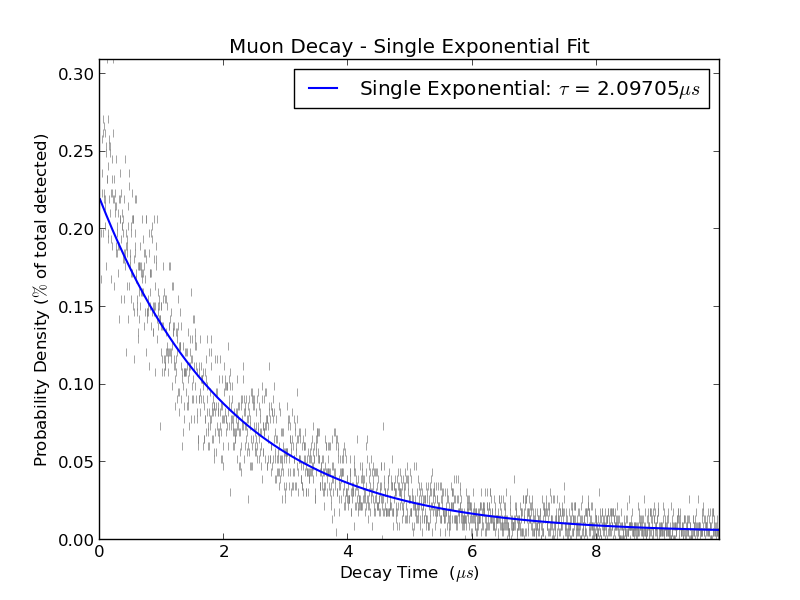
\includegraphics[width=4 in]{graph_EPBB1_SnglExp.png}
\caption{Data Set 1 Single Exponential Fit}
\end{center}
\end{figure}

\begin{figure}[H]
\begin{center}
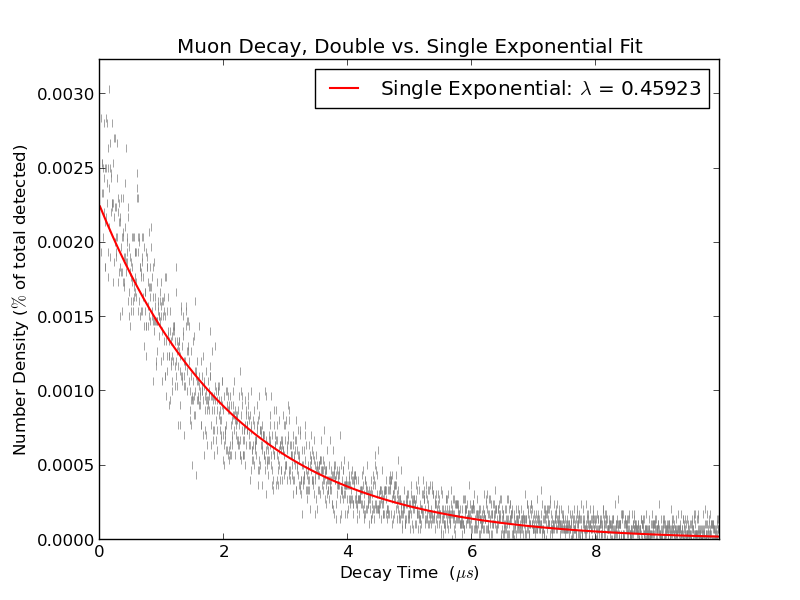
\includegraphics[width=4 in]{graph_EPBB2_SnglExp.png}
\caption{Data Set 2 Single Exponential Fit}
\end{center}
\end{figure}

From the graphs above we can find the decay time from Eq. 3. For the first data set we found a mean lifetime of 2.09705$\mu s \pm 2.12423 \mu s$ and for the second data set we found a mean lifetime of 2.0453 $
\mu s \pm 2.10432 \mu s$.The error on these values is large but this is more a result of the nature of an exponential fit than a real representation of the error.  A much better indicator of the "Goodness of Fit" is the $\chi^2$ level of significance.  This is a statistical tool used to   either reject or accept the fit given. It tests the two hypothesises against each other.\\
\indent \indent $H_0 $: Our parameter values are the true values of the data set.\\
\indent \indent $H_1$: Any other value is the true value of the data set.\\
 For both of our fits the $\chi^2$ significance is at the 77 \% confidence level.  This means that we can accept our $H_0$ hypothesis with this level of confidence.  While this is not great it was the highest level of confidence we were able to achieve.  This is most likely a result of the nature of exponential fits which as opposed to linear fits or unique functions with one or more critical points allow for many similar values to satisfy the fit algorithms requirements.
 
\indent \indent In addition to the lifetime, one of the pertinent fit values is the background parameter C. For our first set of data we found the background to be about 0.0036\% of the total events recorded and for our second set of data we found our background to be 0.0038\% of all events recorded. This is an extraordinary small value and is nearly inconsequential in our data analysis. In further analysis we can increase our $\chi^2$ by subtracting this background from the data set and subsequently eliminate C from our fit parameters. 

\indent \indent The lab manual asks us to calculate the flux per square centimetre  at sea level which we can do for the first set of data since the total run time vs. number of events is known but we cannot find this for the second set of data because we are not sure at which time the apparatus reached the maximum number of events it could record.  Using Eq. 4 and the parameters below we can find the flux detected at sea level.\\
\indent\indent 23315 total events \\
\indent \indent 10,020 min total runtime \\
\indent \indent 3782$ cm^2$ effective detector area. \\
The detected flux in the laboratory is  then roughly 0.00062 events/$cm^2$/min.  This is not anywhere near the accepted flux value at sea level of about 1 event/$cm^2$/min but should not be too concerning because it simply means that our detector does not detect all of the events at sea level. There are several clear reasons for this which are summarized in the list below.
\begin{itemize}
\item The coincidence requirements we have set limit the events we detect to a much smaller sample size. 
\item The effectiveness of the detector varies across its area.
\item We are on the third floor of a large cement and metal structure which may shield a large number of the incident muon shower at sea level. 
\end{itemize} 


\section{Additional Analysis \& Conclusion}
\indent \indent In addition to the single exponential fit asked for in the lab manual we also performed a double exponential fit to account for the fact that muon pairs are produced in cosmic ray showers resulting in the detection of both positive and negative muon decays. Aluminium is a type of exotic atom known as a muonic atom which can capture a negative muon in an inner orbit and eject the farthest valence electron.  The negative muon will maintain this position until it decays following the equation:
\begin{equation}
	\mu^- \rightarrow e^- + \nu_e + \bar{\nu_e}
\end{equation}

\indent \indent We can account for this second decay mode by fitting a double exponential instead of a single exponential to our data.  We did this for both data sets, the figures can be seen below. The equation we are fitting for the double exponential is:
\begin{equation}
P(t) = Ae^{-\alpha t} + Be^{-\beta t} + C
\end{equation}
There are five fit parameters; A and B adjust for the amplitude of the exponential, $\alpha$ and $\beta$ are the inverse of the mean lifetime and C adjusts for background in our measurements. We fit the inverse mean lifetime because it allows for the function to be better defined computationally as well as making the exponential neat by not allowing for division by zero in the argument of the exponential. The initial values for the fit greatly affect the outcome, we attempted many different values but the most successful initial parameters which maximized the $\chi^2$ significance of the data were $\tau = 2.2 \mu s$, $\tau_- = 0.5 \mu s$ and $\tau_+ = 2.2 \mu s$. In a more rigorous examination of the data one would write a routine to maximize $\chi^2$ significance automatically and in a more comprehensive fashion but given the fact we are only analysing two data sets, the guess and check method is perfectly suitable. 

\indent \indent Fig. 4 and Fig. 5 shown below compare the double exponential v. the single exponential fit and shows the calculated mean decay times.  As you can see the functional form is not graphically very different but the decay times are significantly different.  It should be noted that the uncertainty in the double exponential fit values is enormously large.  This is because there are a large variety of linear combinations of exponentials which can satisfy the needed functional form.  The error is so large as to make the values given in the graphs statistically insignificant. This should be treated merely as an exercise since from our perspective positive and negative muons are not well differentiated in our data set. Without the foresight of knowing that there are two different decay modes being observed our experimental analysis would not allow us to be confident that our double exponential fit was meaningful.    

\begin{figure}[H]
\begin{center}
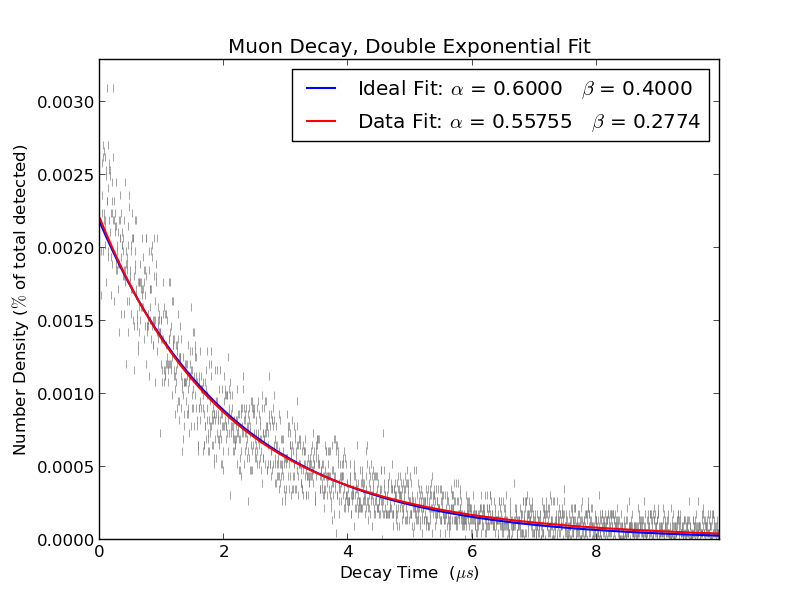
\includegraphics[width=4 in]{graph_EPBB1_DbleExp.png}
\caption{Data Set 1 Double V. Single Exponential Fit}
\end{center}
\end{figure}

\begin{figure}[H]
\begin{center}
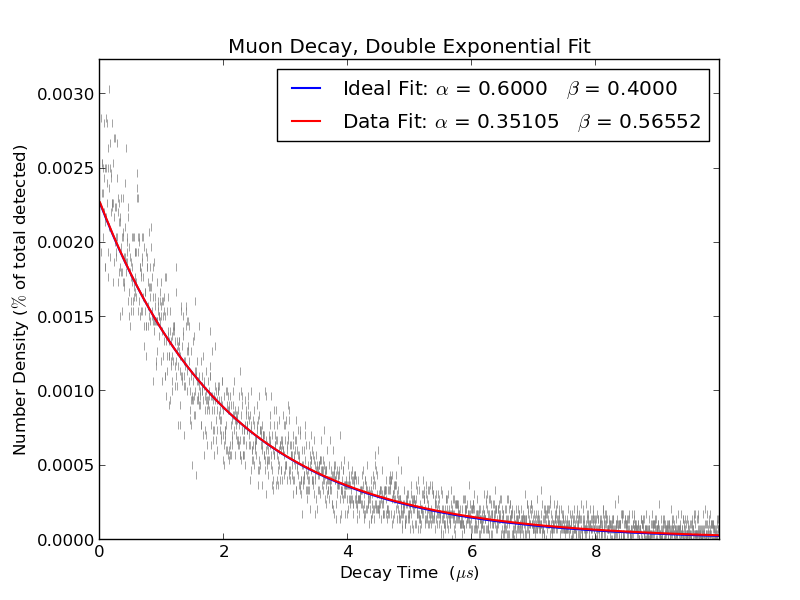
\includegraphics[width=4 in]{graph_EPBB2_DbleExp.png}
\caption{Data Set 2 Double V. Single Exponential Fit}
\end{center}
\end{figure} 

\indent \indent In order to emphasize the importance of including both decay paths in our fit Fig. 6 and Fig. 7 separate out the respective contributions to our fit from the positive and negative muon decays. 

\begin{figure}[H]
\begin{center}
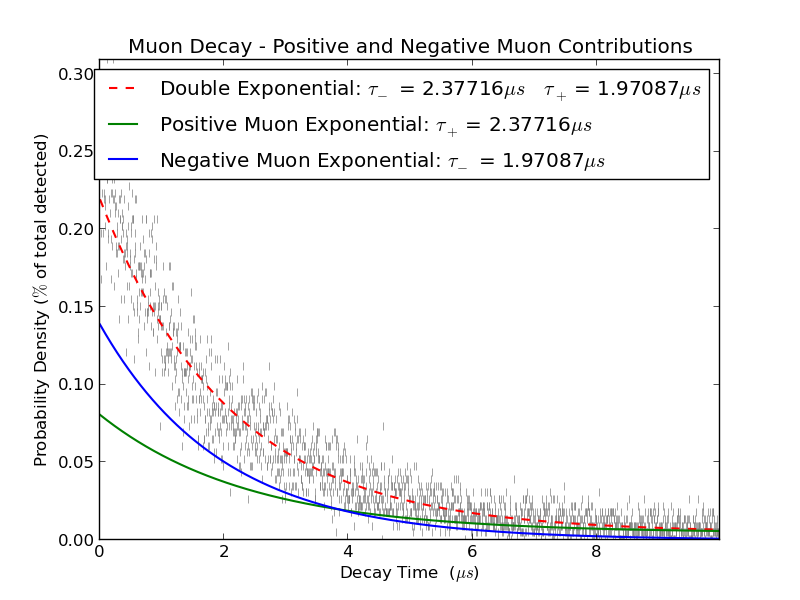
\includegraphics[width=4 in]{graph_EPBB1_CompExp.png}
\caption{Data Set 1 Positive and Negative Contributions to Fit}
\end{center}
\end{figure}

\begin{figure}[H]
\begin{center}
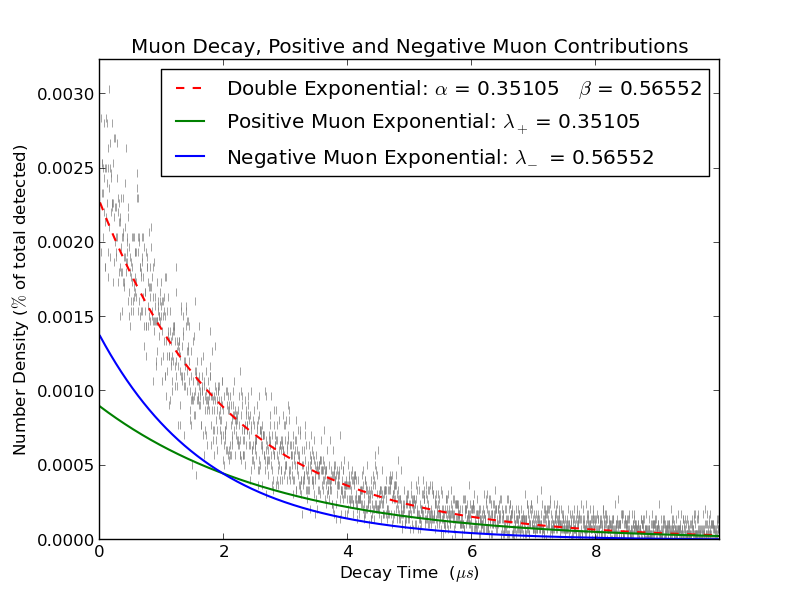
\includegraphics[width=4 in]{graph_EPBB2_CompExp.png}
\caption{Data Set 2 Positive and Negative Contributions to Fit}
\end{center}
\end{figure}

As can be seen from the above figures the positive muon decay is dominant in the longer decay times while the negative muon due to absorption into the aluminium atom is dominant in the shorter decay times.  

The full fitting routine is available online at the GitHub repository provided in the references section  \cite{Fitting}.


\begin{thebibliography}{99}
\bibitem{electron}Sleator, Tycho, and Budick, Burton, \begin{em}Muon Lifetime. \end{em}Experimental Physics. V85.0112. Spring, 2012.
\bibitem{LabTools} LabTools Public Documentation -  \emph{http://wanda.fiu.edu/boeglinw/LabTools/doc/index.html}
\bibitem{Fitting} \emph{http://www.github.com} 
\\     User: BoothDunbar-Brandon \\       Public Repository: Advanced-Experimental/muon-lifetime/smartmuon.py
\end{thebibliography}

\newpage \LARGE{Appendix}

\end{document}  
